\section{Reamostragem Por Importância Sequencial (SIR)}\label{sir}

Como uma das aproximações estocásticas a serem consideradas, o método da reamostragem por importância sequencial (SIR), ou reamostragem ponderada, foi uma das primeiras alternativas aos métodos de aproximação determinísticos previamente existentes. Se antes a densidade conjunta era aproximada por uma regra de quadratura, nas aproximações estocásticas o objetivo é simular amostras de uma densidade que aproxime a desejada com o menor erro possível. Este erro dependerá de $k$, o tamanho de uma amostra retirada da densidade aproximada, de ordem $\mathcal{O}(k^{-1})$, e não mais do conjunto de dados amostrais do modelo inicial.

Proposto por Gordon \textit{et al.} (1993)\cite{Gordon1993}, o método SIR utiliza uma \textit{função de amostragem por importância} $g$ para aproximar (sem perda de generalidade) uma densidade de interesse $p$. Neste caso, $g$ é uma densidade conhecida e da qual se sabe gerar uma amostra aleatória. Cada ponto selecionado na amostra de $g$ é ponderado para corrigir a probabilidade de amostragem de tal forma que a amostra ponderada aproxime uma outra que seria extraída da densidade de $p$ caso se soubesse gerar da mesma. Os pesos usados para corrigir as probabilidades de amostragem são chamados \textit{pesos de importância padronizados}. Sejam $\theta_1, \ldots, \theta_t$ uma amostra aleatória de $g$ e $\bm{y}$ uma amostra do modelo para os dados observados. Para cada ponto $\theta_j$, $j = 1, \ldots, t$, os pesos são dados por
\begin{equation}\label{eq:sir_wei}
w_j(\theta_j) = \dfrac{p(\theta_j | \bm{y}) / q(\theta_j)}{\sum_{j=1}^{t} p(\theta_j | \bm{y}) / q(\theta_j)}.
\end{equation}

Após gerar $t$ valores $w_j(\theta_j)$, uma reamostragem de tamanho $k$ é feita do suporte discreto $\theta_1, \ldots, \theta_t$ com probabilidades $w_1(\theta_1), \ldots, w_t(\theta_t)$. A nova amostra resultante terá uma distribuição aproximadamente igual à de $p$, convergindo para esta quando $t \rightarrow \infty$ se $k$ é fixo ou quando $t/m \rightarrow 0$. Em geral, é suficiente que $k/t = 1/10$, razão que será utilizada em todos os cenários ($t$ será $10$ vezes o valor de $k$). Logo, o método SIR gera uma amostra de $p$ assintoticamente. Observe que a densidade $g$ a ser escolhida deve ter o mesmo suporte de $p$ para que o método funcione.

No presente trabalho, tem-se 3 parâmetros ($\mu, \sigma^2$ e $\nu$) a serem gerados dada uma densidade \textit{a posteriori} $p(\mu, \sigma^2, \nu | \bm{x})$. Como esta densidade possui uma constante de proporcionalidade $c$ associada, pela razão do lado direito de \eqref{eq:sir_wei} esta é cancelada, sendo possível trabalhar apenas com o núcleo de $p(\mu, \sigma^2, \nu | \bm{x})$ calculado no lado direito em \eqref{eq:dist_post}. Isto por si só é uma vantagem do método SIR em relação à quadratura de Riemann, para a qual se viu que era necessário aproximar $c$. Como se deseja aproximar uma função conjunta de 3 parâmetros, a densidade $g$ a ser escolhida deve não apenas ter a mesma dimensão, mas também cada uma de suas componentes marginais deve ter o mesmo suporte do parâmetro correspondente no núcleo de $p(\mu, \sigma^2, \nu | \bm{x})$.

\begin{figure}[t]%
	\centering
	\subfloat[Histograma de $\mu$]{{
			\label{fig:mu_sir_500}
			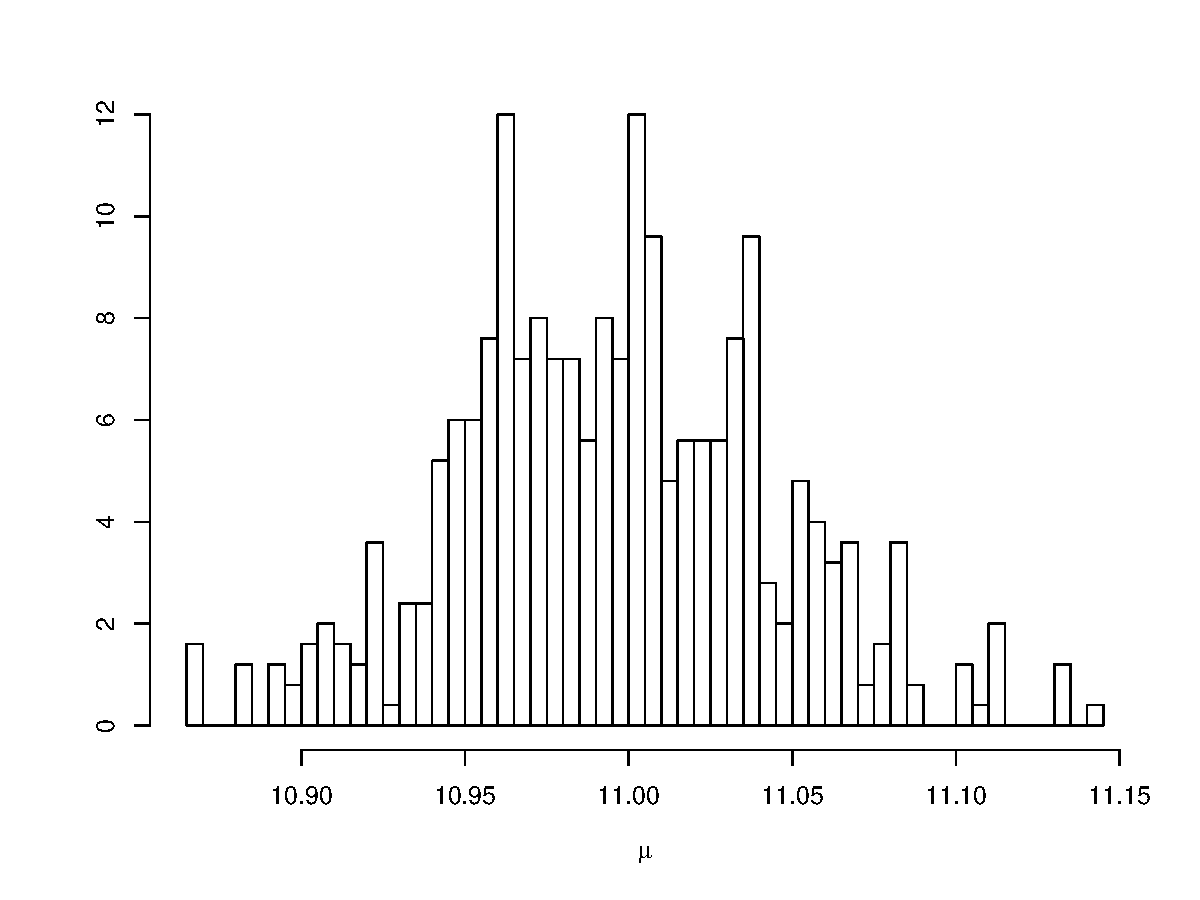
\includegraphics[scale=0.4]{figuras/mu_sir_500.pdf}}}%
	\qquad
	\subfloat[Histograma de $\sigma^2$]{{
			\label{fig:s2_sir_500}
			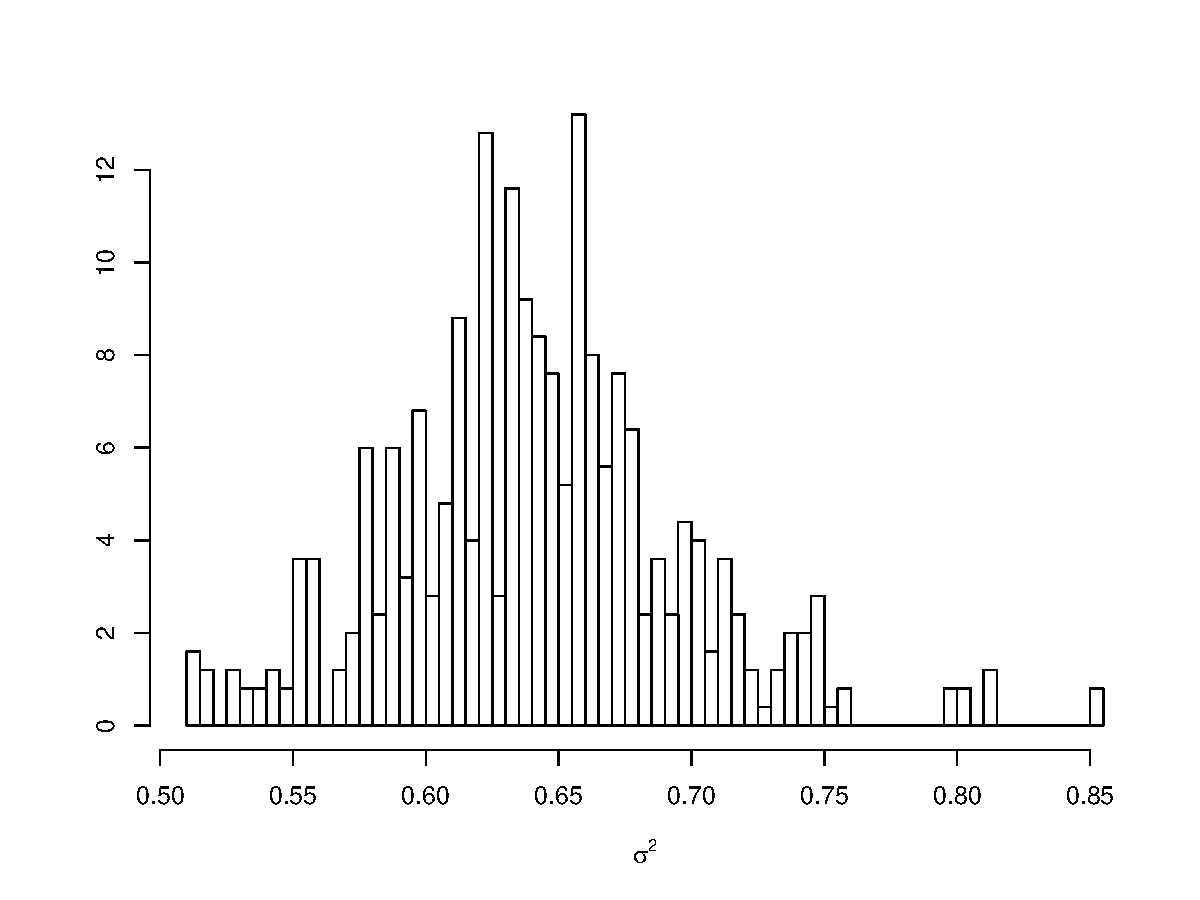
\includegraphics[scale=0.4]{figuras/s2_sir_500.pdf}}}%
	\subfloat[Histograma de $\nu$]{{
			\label{fig:nu_sir_500}
			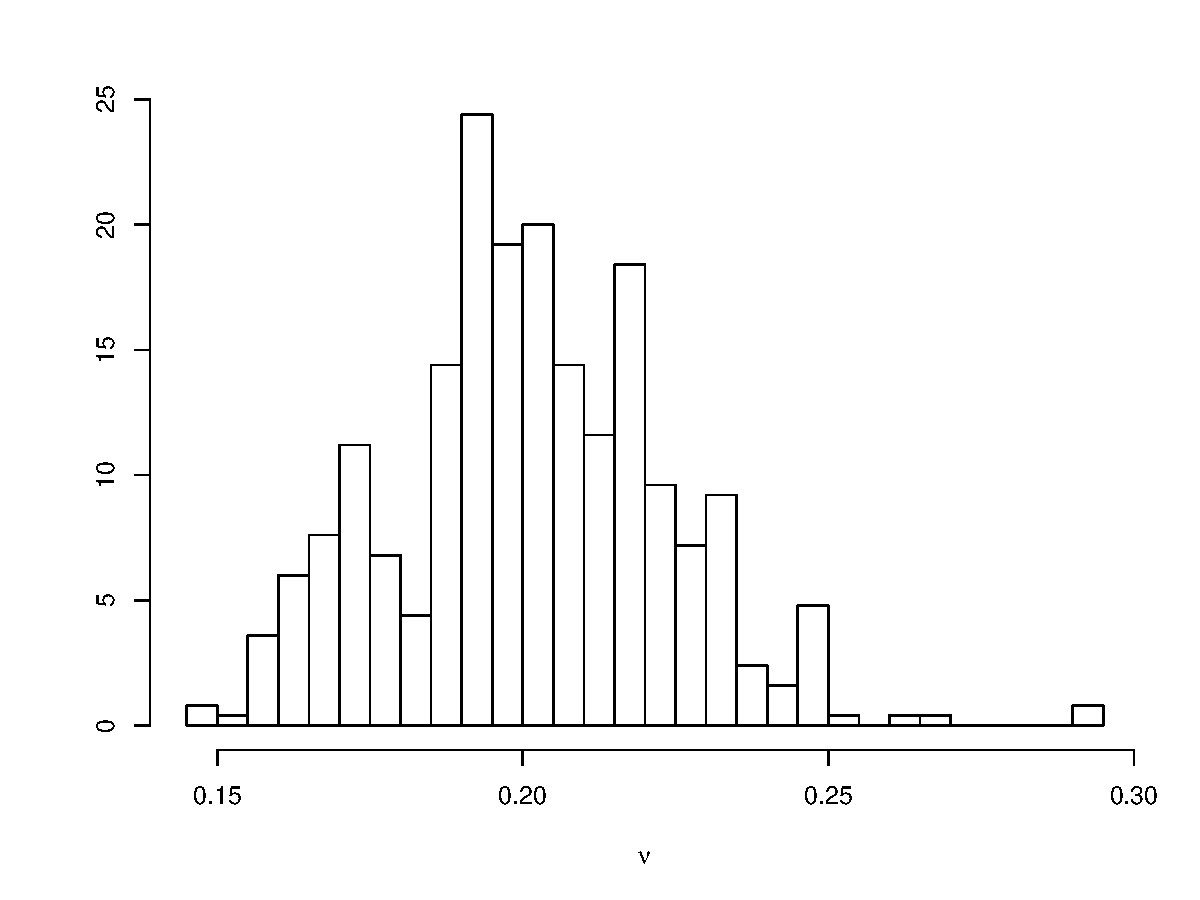
\includegraphics[scale=0.4]{figuras/nu_sir_500.pdf}}}%
	\caption{Histograma das densidades \textit{a posteriori} marginais pelo método SIR com $k = 500$}%
\end{figure}

Como feito em muitos trabalhos, para $g$ será escolhida uma densidade normal trivariada $N_3(\bm{\mu}, \bm{\Sigma})$, cujas componentes têm, cada uma, suporte em toda a reta real. Note que para 2 parâmetros, $\sigma^2$ e $\nu$, o respectivo espaço paramétrico não é a reta real ($\Theta_{\sigma^2} = \mathbb{R}_+$ e $\Theta_{\nu} = [0,1]$, respectivamente). Desta forma, antes de usar o método é necessário reparametrizar \eqref{eq:dist_post} de modo que todos os novos parâmetros tenham suporte em $\mathbb{R}$. Para a reparametrização, consideram-se as transformações $\theta_1 = \mu, \theta_2 = \log(\sigma^2)$ e $\theta_3 = \log[\nu/(1-\nu)]$. Logo, a expressão do núcleo reparametrizado é dada por
\begin{align}
p(\theta_1, \theta_2, \theta_3 | \bm{x})
&= p(\theta_1 = \mu, \theta_2 = \log(\sigma^2), \theta_3 = \log[\nu/(1-\nu)] | \bm{x}) \nonumber \\
&= p(\mu = \theta_1, \sigma^2 = \exp(\theta_2), \nu = 1/[1 + \exp(-\theta_3)] | \bm{x}) \times |J(\theta_1, \theta_2, \theta_3)| \nonumber \\
&\propto \left[\exp(\theta_2)\right]^{-[(n + 1)/2 + a + 1]} \times \exp\left\{-\dfrac{\left[(\theta_1 - m)^2 / (2V) + d\right]}{\exp(\theta_2)}\right\} \nonumber \\
&\times A^*(\bm{x} | \theta_1, \theta_2, \theta_3) \times  \dfrac{\exp(\theta_2) \exp(\theta_3)}{\left[1 + \exp(-\theta_3)\right]^{-2}} \nonumber
\end{align}

\begin{align}
\Rightarrow p(\theta_1, \theta_2, \theta_3 | \bm{x}) &\propto \left(\dfrac{1}{\sigma^2}\right)^{(n + 1)/2 + a + 1} \times \exp\left\{-\dfrac{\left[(\mu - m)^2 / (2V) + d\right]}{\sigma^2}\right\} \times A(\bm{x} | \mu, \sigma^2, \nu) \nonumber \\
&\times \sigma^2 \nu^3(1-\nu)^{-1}, \label{eq:sir_dpre}
\end{align}
onde $|J(\theta_1, \theta_2, \theta_3)|$ é o determinante da matriz jacobiana das derivadas parciais de $(\mu, \sigma^2, \nu)$ com respeito a $(\theta_1, \theta_2, \theta_3)$. No cálculo deste determinante, todos os elementos fora da diagonal principal da matriz jacobiana serão nulos, já que na reparametrização utilizada não se assumiu nenhuma função dependente de mais de um parâmetro.

\begin{figure}[t]%
	\centering
	\subfloat[Histograma de $\mu$]{{
			\label{fig:mu_sir_5000}
			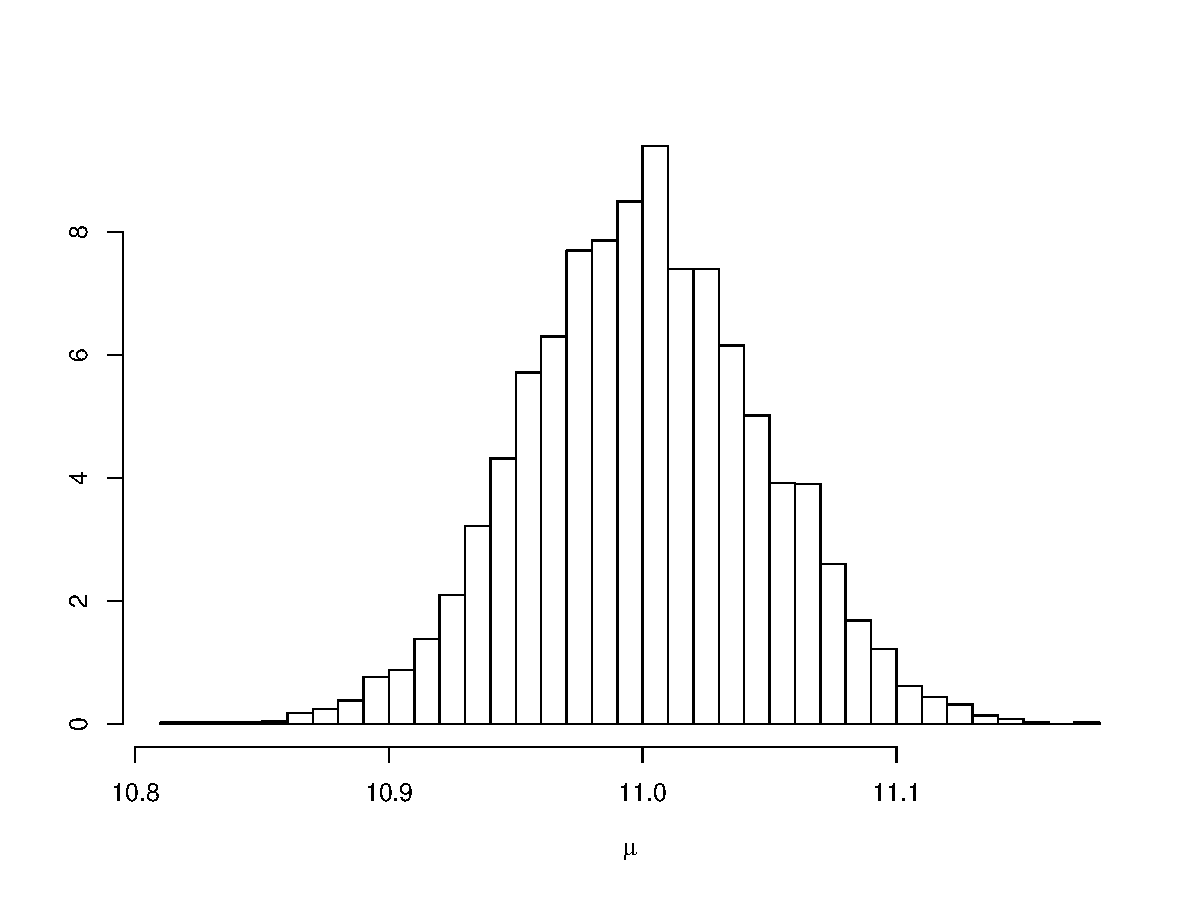
\includegraphics[scale=0.4]{figuras/mu_sir_5000.pdf}}}%
	\qquad
	\subfloat[Histograma de $\sigma^2$]{{
			\label{fig:s2_sir_5000}
			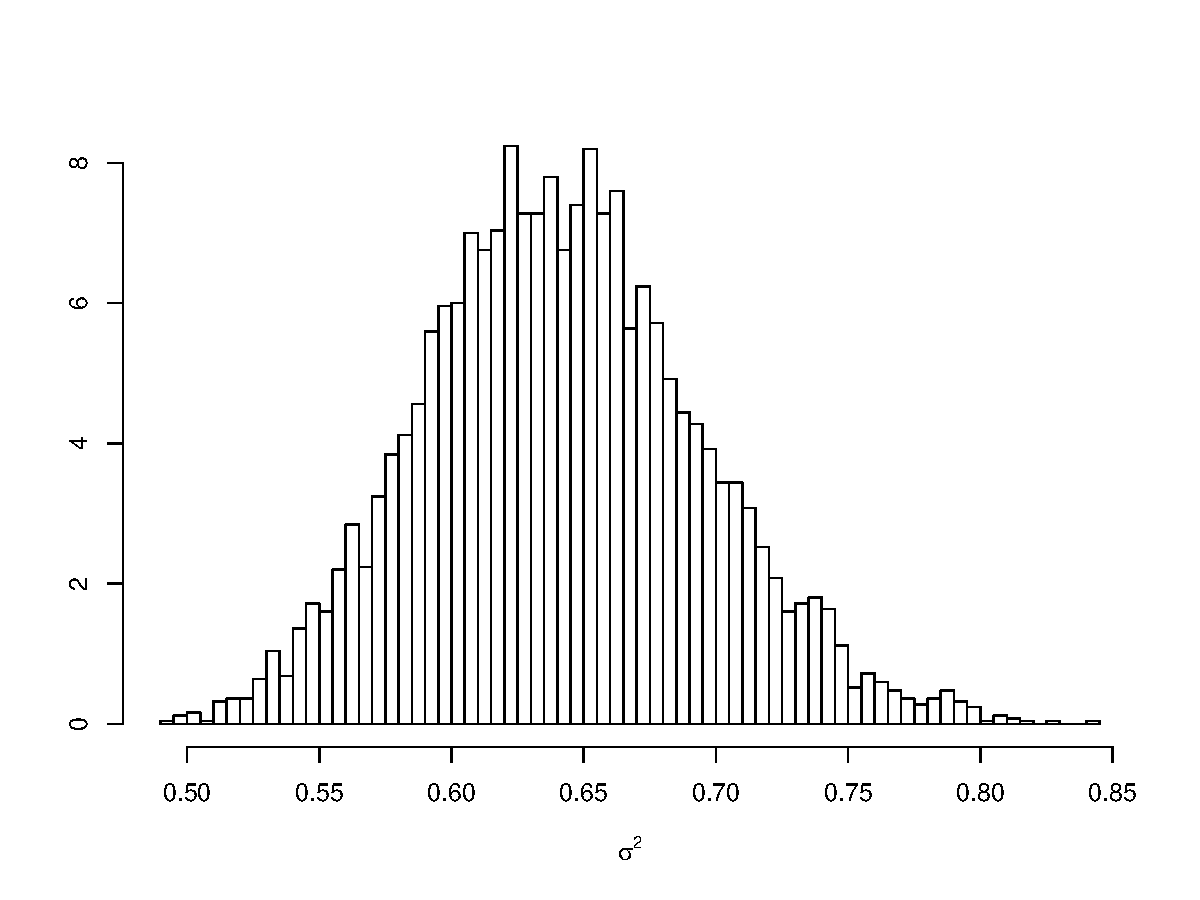
\includegraphics[scale=0.4]{figuras/s2_sir_5000.pdf}}}%
	\subfloat[Histograma de $\nu$]{{
			\label{fig:nu_sir_5000}
			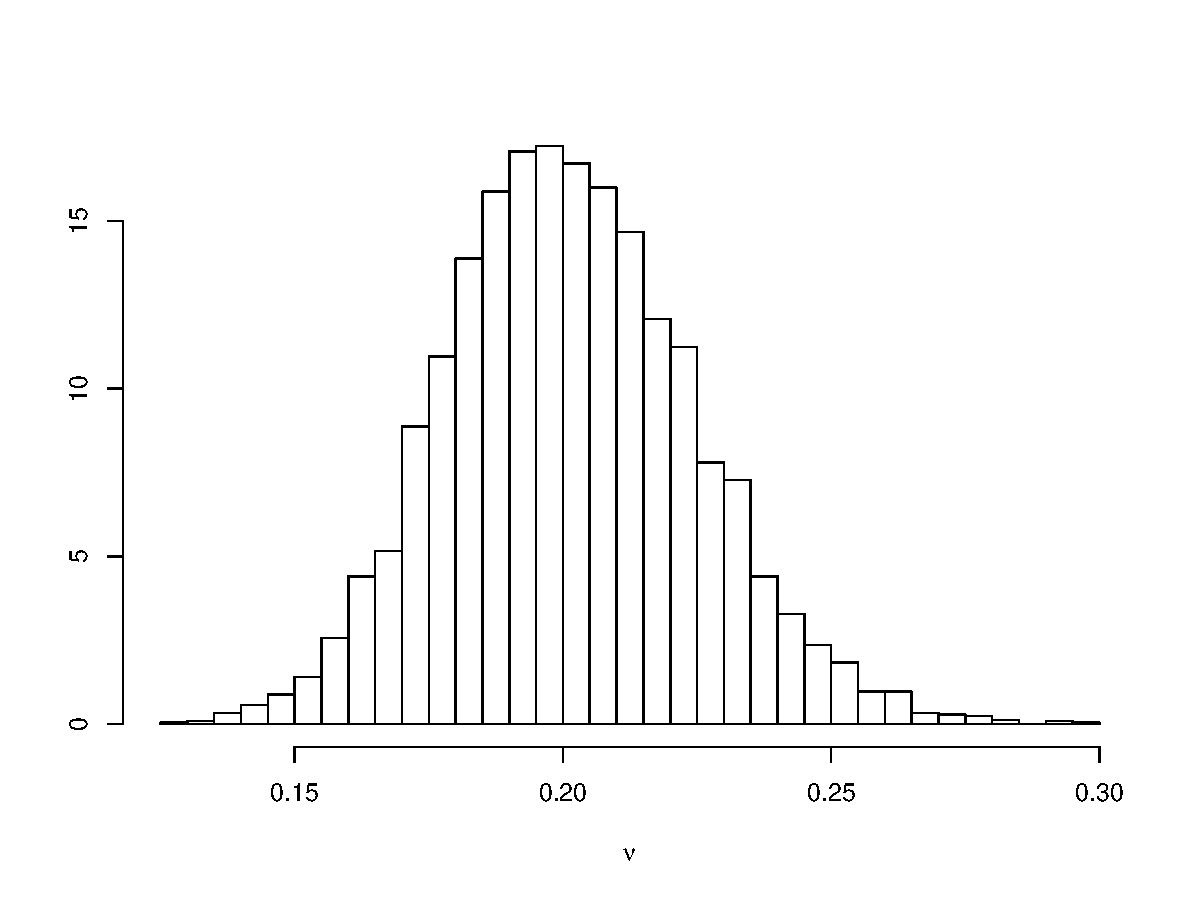
\includegraphics[scale=0.4]{figuras/nu_sir_5000.pdf}}}%
	\caption{Histograma das densidades \textit{a posteriori} marginais pelo método SIR com $k = 5000$}%
\end{figure}

\begin{figure}[t]%
	\centering
	\subfloat[Histograma de $\mu$]{{
			\label{fig:mu_sir_50000}
			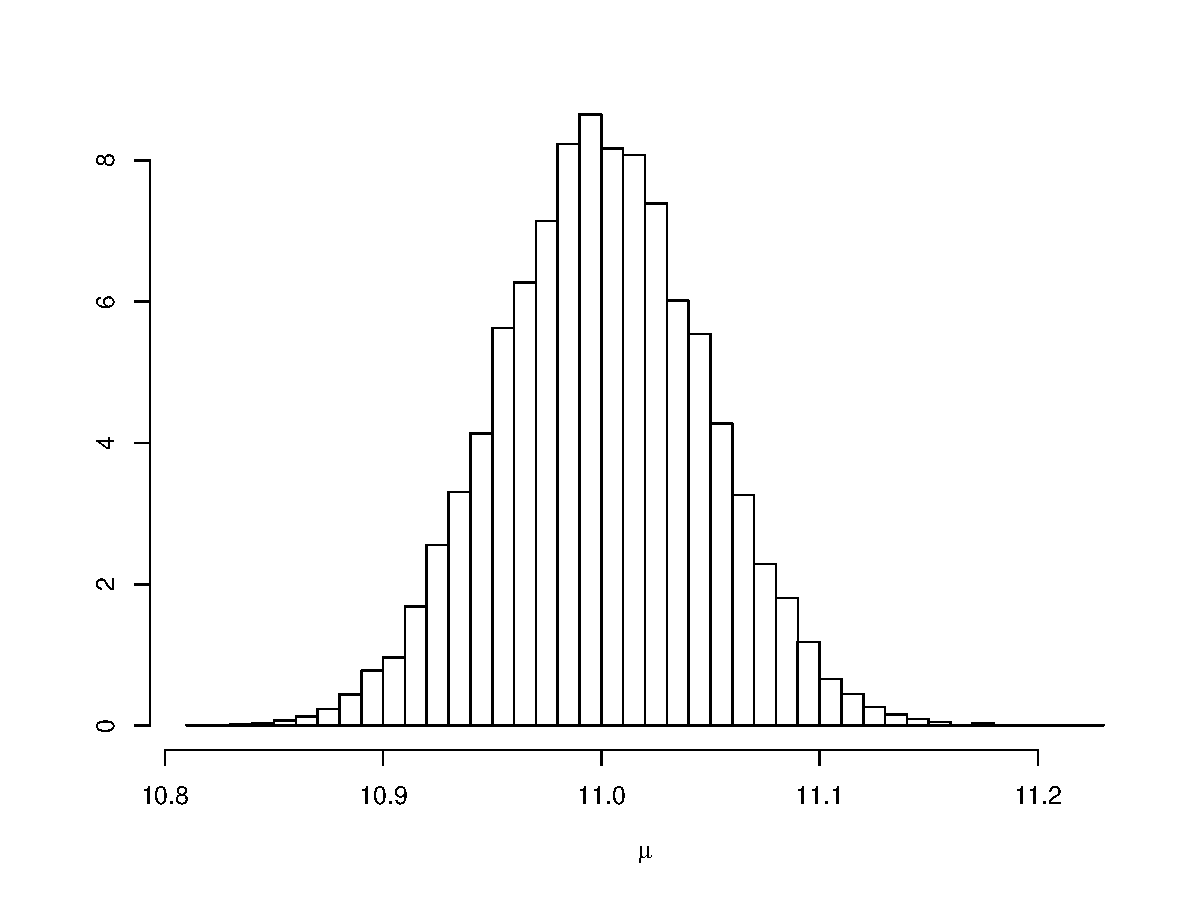
\includegraphics[scale=0.4]{figuras/mu_sir_50000.pdf}}}%
	\qquad
	\subfloat[Histograma de $\sigma^2$]{{
			\label{fig:s2_sir_50000}
			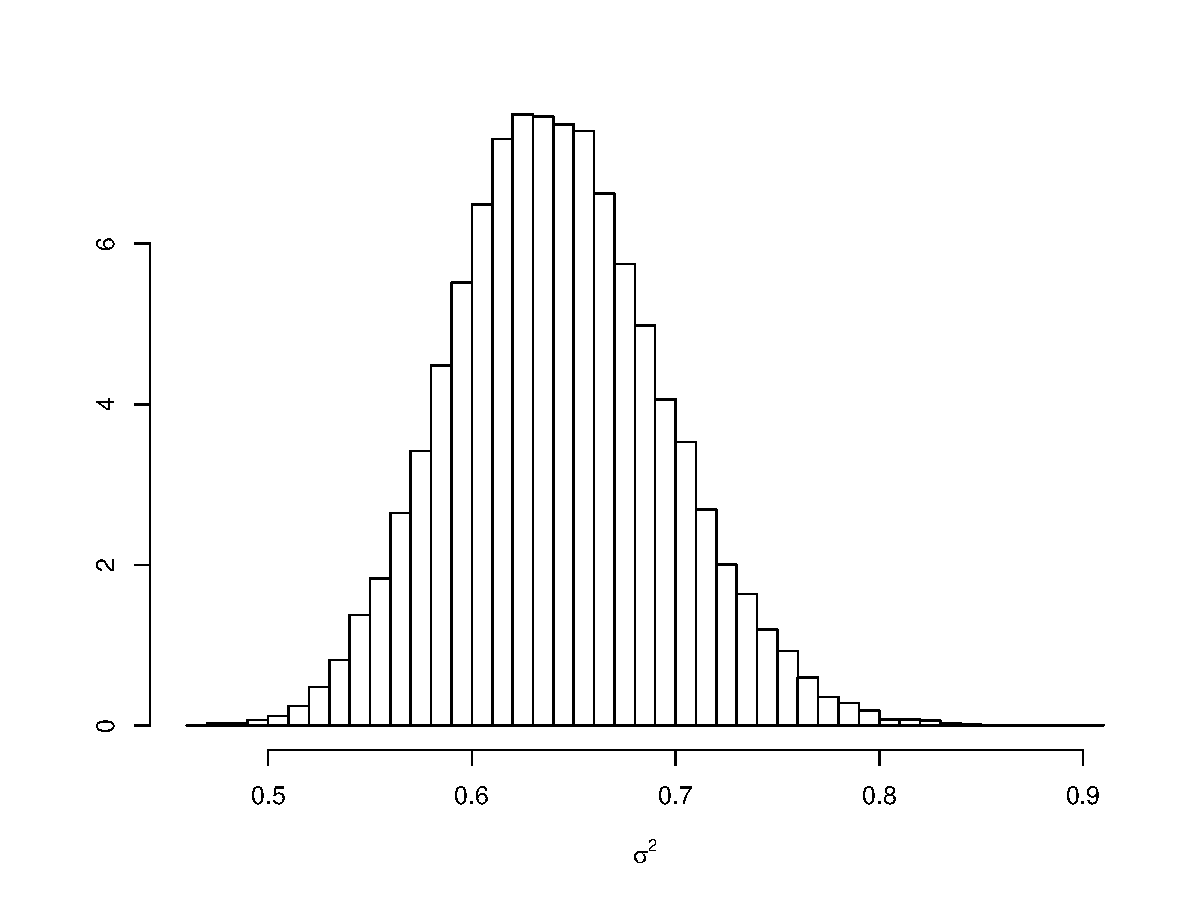
\includegraphics[scale=0.4]{figuras/s2_sir_50000.pdf}}}%
	\subfloat[Histograma de $\nu$]{{
			\label{fig:nu_sir_50000}
			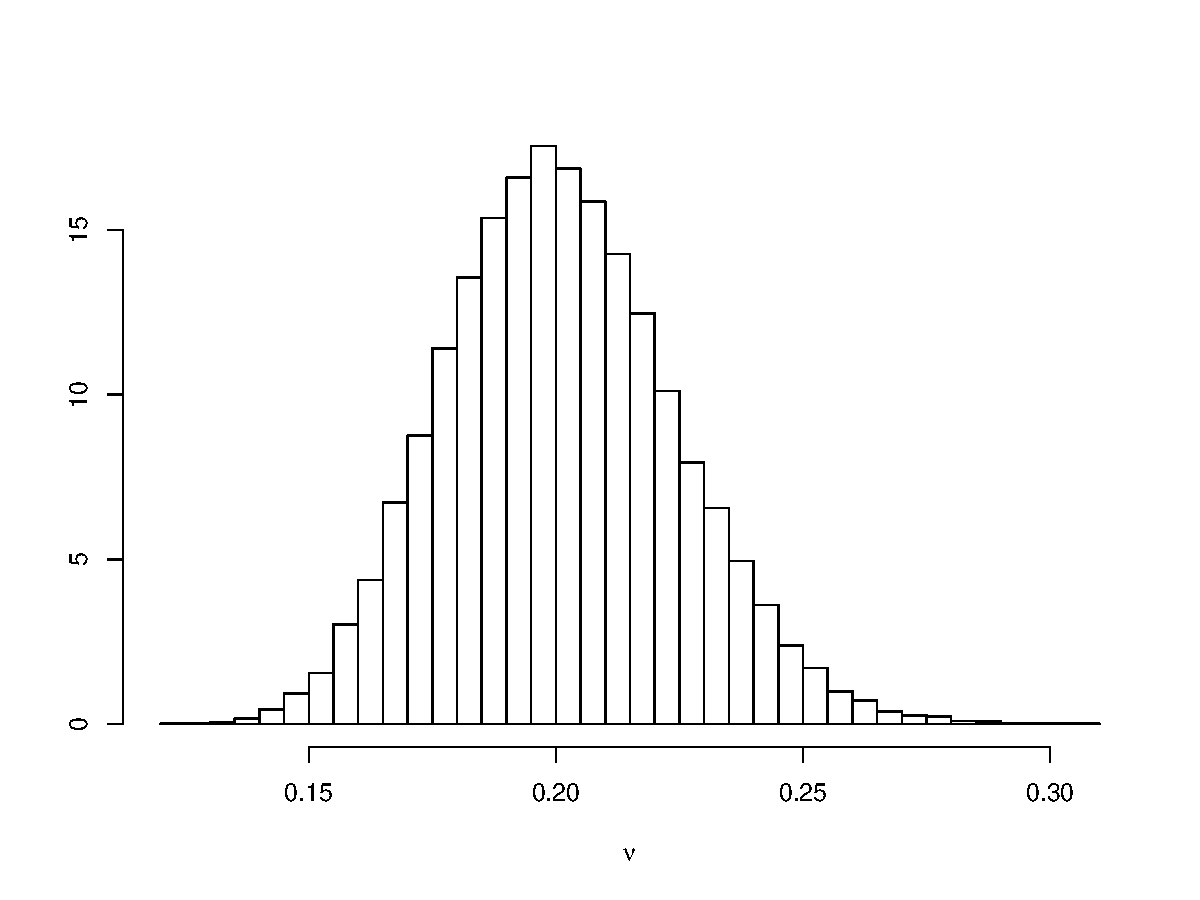
\includegraphics[scale=0.4]{figuras/nu_sir_50000.pdf}}}%
	\caption{Histograma das densidades \textit{a posteriori} marginais pelo método SIR com $k = 50000$}%
\end{figure}

Novamente, para a versão reparametrizada do núcleo da densidade em \eqref{eq:sir_dpre} deve-se primeiro tomar o logaritmo de cada termo em seu produto para só depois exponenciá-la, de modo a evitar problemas numéricos. Para a amostra de tamanho $n=500$ da mistura finita de normais com variância contaminada tal que $\mu = 11$; $\sigma^2 = 0.64$; $\nu = 0.2$; $m = 11$; $V = 1$; $a = 7$ e $d = 4$ (Figura \ref{fig:sample_n.pdf}), o logaritmo do núcleo da densidade \textit{a posteriori} reparametrizada é igual a $-523.9575$ (bem próximo do valor na parametrização original), cuja exponencial é aproximadamente igual a $2.806 \times 10^{-228}$.

Os gráficos das densidades \textit{a posteriori} marginais para cada parâmetro quando os demais são fixados nos seus valores verdadeiros (Figuras \ref{fig:maspro_mu} a \ref{fig:maspro_nu}), os quais fornecem os respectivos intervalos de massa probabilística, novamente serão úteis, mas agora para definir a parametrização da distribuição normal trivariada a ser usada no método SIR. Para as médias das componentes desta distribuição, será fixado $\bm{\mu} = (\theta_1, \theta_2, \theta_3) = (\mu, \log(\sigma^2), \log[\nu/(1-\nu)]) = (11, \log(0.64), \log[0.2/0.8])$. Para a matriz de covariância $\bm{\Sigma}$, cada elemento da diagonal principal será dado pelo quadrado de $1/6$ do intervalo de massa probabilística do parâmetro correspondente. Esta escolha se justifica pelo fato de que as distribuições mostradas de \ref{fig:maspro_mu} a \ref{fig:maspro_nu} têm comportamento próximo à normalidade. Para uma distribuição normal, $99.7\%$ de sua massa probabilística está concentrada a até uma distância de 3 vezes o seu desvio padrão em relação ao ponto médio. Para os elementos fora da diagonal principal de $\bm{\Sigma}$, todos foram assumidos iguais a zero. Desta forma, $\bm{\Sigma} = \textrm{diag}\{0.0022, 0.0065, 0.0203\}$.

Escolhida a densidade $g$, resta aplicar o método SIR para obter amostras \textit{a posteriori} de $\mu$, $\sigma^2$ e $\nu$. Para este trabalho, foram considerados 3 cenários: $k = \{500, 5000, 50000\}$. Em cada cenário, foram geradas amostras de cada componente de $g$. Cada ponto amostral foi reparametrizado (quando fosse o caso) de volta para obter os valores estimados de $\mu$, $\sigma^2$ e $\nu$. Por fim, para todos os pontos amostrais de $g$ também foi calculado o valor da densidade conjunta, necessária para obter os pesos de importância padronizados do método SIR. Construído o suporte discreto para cada parâmetro a partir dos pontos amostrais da componente de $g$ correspondente, amostras \textit{a posteriori} são obtidas associando cada peso ao ponto amostral correspondente de $g$. Nas figuras \ref{fig:mu_sir_500} a \ref{fig:nu_sir_500}; \ref{fig:mu_sir_5000} a \ref{fig:nu_sir_5000} e \ref{fig:mu_sir_50000} a \ref{fig:nu_sir_50000} são apresentados os histogramas para as amostras \textit{a posteriori} de cada parâmetro por cenário.

Para $k=500$, a aproximação da densidade não é boa para nenhum dos 3 parâmetros: há alguns pontos extremos (em inglês, \textit{outliers}) distantes do que seria a massa principal, especialmente para $\sigma^2$ e $\nu$. Além disso, há vários pontos de máximo locais (modas), indicando uma curva longe de ser suave. Entretanto, é possível dizer já neste cenário como é o comportamento de cada parâmetro com relação à locação.

Para $k=5000$, a aproximação é muito mais suave e há bem menos \textit{outliers}. O número de modas locais também é severamente reduzido em comparação ao cenário anterior, embora esta quantidade ainda seja moderada para $\sigma^2$. Além do comportamento com relação à locação, é possível dizer também como é o comportamento com relação à dispersão e à simetria da densidade \textit{a posteriori} marginal de cada parâmetro. Aparentemente, as densidades para $\sigma^2$ e $\nu$ são fracamente assimétricas à direita.

Para $k=50000$, os gráficos confirmam a tendência apresentada pelo cenário anterior, mas com uma suavização ainda melhor. Agora, todas as distribuições são unimodais e não há mais \textit{outliers}. Computacionalmente, a reamostragem é um pouco mais demorada, mas não na mesma taxa da quadratura de Riemann, já que agora o número de pontos amostrais cresce a um fator de ordem $\mathcal{O}(k)$, logo de modo linear.

Obtidas as amostras \textit{a posteriori} marginais de cada parâmetro, para aproximar as estatísticas de média, variância, assimetria e curtose é suficiente que se tomem as respectivas estimativas amostrais. Na Tabela \ref{tab2}, são apresentados os valores aproximados para tais estatísticas em cada um dos três cenários.

\begin{table}[t]
	\caption{Estatísticas \textit{a posteriori} para $(\mu, \sigma^2, \nu)$ pelo método SIR}
	\label{tab2}
	\centering
	\begin{tabular}{cccccc}
		\toprule
		Cenário & Parâmetro & Média & Variância & Assimetria & Curtose \\
		\midrule
		$k = 500$ & $\mu$      & 11.0003 & 0.0023 & -0.0610 & 3.0351 \\
		          & $\sigma^2$ &  0.6422 & 0.0026 &  0.1261 & 3.1453 \\
		          & $\nu$      &  0.2028 & 0.0006 &  0.3510 & 3.5475 \\
		\midrule
		$k = 5000$ & $\mu$      & 11.0006 & 0.0022 &  0.0216 & 3.0234 \\
		           & $\sigma^2$ &  0.6418 & 0.0027 &  0.2349 & 3.0118 \\
		           & $\nu$      &  0.2013 & 0.0005 &  0.2485 & 3.1646 \\
		\midrule
		$k = 50000$ & $\mu$      & 11.0002 & 0.0022 & -0.0081 & 3.0451 \\
		            & $\sigma^2$ &  0.6420 & 0.0027 &  0.2353 & 3.1153 \\
		            & $\nu$      &  0.2009 & 0.0005 &  0.2608 & 3.0849 \\
		\bottomrule
	\end{tabular}
\end{table}

Pela Tabela \ref{tab2}, pode-se concluir que tanto a média quanto a variância \textit{a posteriori} variaram muito pouco nos três cenários, independente do parâmetro considerado. Isto quer dizer que amostras \textit{a posteriori} de tamanho moderado são o suficiente para se obter uma boa aproximação destas duas estatísticas. Por outro lado, o mesmo não pode ser dito para a assimetria e curtose \textit{a posteriori}, para as quais há grandes mudanças inclusive na primeira casa decimal, mesmo de $k=5000$ para $k=50000$. Assim como na quadratura de Riemann, isto se explica pelo fato de que tanto a assimetria quanto a curtose são funções que dependem de vários momentos, até a terceira e quarta ordem respectivamente. Apesar deste fato, também no método SIR se pode dizer que houve uma estabilidade nas aproximações destas duas últimas estatísticas na medida em que $k$ crescia.

Com relação aos valores em si, as médias \textit{a posteriori} para os 3 parâmetros coincidiram, até a terceira casa decimal, com os respectivos valores do modelo para a distribuição amostral. Desta forma, as médias \textit{a posteriori} aproximadas pelo método SIR estão mais próximas dos valores no modelo do que as obtidas na Tabela \ref{tab1} pela quadratura de Riemann. Para as variâncias \textit{a posteriori}, todas elas foram bem pequenas, em especial para $\nu$, assim como na quadratura.

Com relação à assimetria \textit{a posteriori}, esta foi praticamente nula para $\mu$ e positiva, mas fraca, para $\sigma^2$ e $\nu$ (um pouco mais forte para a segunda, ao contrário da conclusão para a quadratura). Por fim, as aproximações para a curtose \textit{a posteriori} foram todas bem próximas de 3 (desta vez, acima deste valor), o valor encontrado para uma distribuição normal, com o parâmetro $\mu$ mais próximo desse valor e $\sigma^2$ o mais afastado, um pouco diferente do que foi encontrado para a quadratura.